\section{IHS Markit dataset}

The IHS Markit dataset provides valuable vessel specification data for big data analysis in maritime shipping.
This dataset offers comprehensive information on vessel characteristics, including dimensions, tonnage, engine capacity, and ownership.
By leveraging this dataset, researchers can gain insights into the diverse specifications of vessels operating in the maritime industry.

Analyzing vessel specifications from the IHS Markit dataset allows for a deeper understanding of the maritime shipping landscape.
Researchers can explore correlations between vessel characteristics and various factors such as fuel efficiency, cargo capacity, or operational performance.
These insights can aid in optimizing vessel selection, fleet management, and decision-making processes related to vessel operations.

By utilizing the vessel specification data from the IHS Markit dataset, this research contributes to enhancing operational efficiency and optimizing vessel-related decisions in the maritime shipping industry.
This dataset equips this research to identify trends and patterns in the maritime shipping industry related to vessel characteristics.
This comprehensive dataset serves as a robust foundation for my research, enabling me to draw meaningful conclusions and make data-driven recommendations for the future of the industry.

\begin{figure}[h]
    \centering
    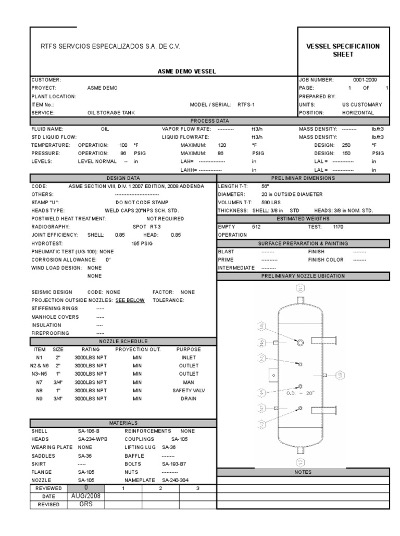
\includegraphics[width=0.5\textwidth]{images/vessel_specification.jpg}
    \caption{Vessel Specification Sheet \autocite{Itur}}
    \label{vessel_specification}
\end{figure}